\documentclass[12pt]{article}
\usepackage[margin=2.5cm]{geometry}
\usepackage{enumerate}
\usepackage{amsfonts}
\usepackage{amsmath}
\usepackage{fancyhdr}
\usepackage{amsmath}
\usepackage{amssymb}
\usepackage{amsthm}
\usepackage{mdframed}
\usepackage{graphicx}
\usepackage{subcaption}
\usepackage{adjustbox}
\usepackage{listings}
\usepackage{xcolor}
\usepackage{booktabs}
\usepackage[utf]{kotex}
\usepackage{hyperref}

\definecolor{codegreen}{rgb}{0,0.6,0}
\definecolor{codegray}{rgb}{0.5,0.5,0.5}
\definecolor{codepurple}{rgb}{0.58,0,0.82}
\definecolor{backcolour}{rgb}{0.95,0.95,0.92}

\lstdefinestyle{mystyle}{
    backgroundcolor=\color{backcolour},
    commentstyle=\color{codegreen},
    keywordstyle=\color{magenta},
    numberstyle=\tiny\color{codegray},
    stringstyle=\color{codepurple},
    basicstyle=\ttfamily\footnotesize,
    breakatwhitespace=false,
    breaklines=true,
    captionpos=b,
    keepspaces=true,
    numbers=left,
    numbersep=5pt,
    showspaces=false,
    showstringspaces=false,
    showtabs=false,
    tabsize=1
}

\lstset{style=mystyle}

\pagestyle{fancy}
\renewcommand{\headrulewidth}{0.4pt}
\lhead{Team Treehouse}
\rhead{Java Basics Part 1 Notes}

\begin{document}
\title{Java Basics Part 1 Notes}
\author{Team Treehouse}
\maketitle

\section{Introuction to Your Tools}
\section{Quiz 1}

\bigskip

\begin{enumerate}[1.]
    \item

    Single line comments in Java begins with the following characters

    \bigskip

    \begin{enumerate}[A.]
        \item `**'
        \item ??
        \item //
        \item $\backslash\backslash$
        \item None of the above
    \end{enumerate}

    \bigskip

    \textbf{Answer:} C

    \item

    The command line tool that is used to compile your program is

    \bigskip

    \begin{enumerate}[A.]
        \item java
        \item compile
        \item ls
        \item javac
    \end{enumerate}

    \bigskip

    \textbf{Answer:} D

    \item Single line comments in Java begin with the following characters

    \bigskip

    \begin{enumerate}[A.]
        \item java
        \item compile
        \item ls
        \item javac
    \end{enumerate}

    \item

    Java is a compiled language

    \bigskip

    \begin{enumerate}[A.]
        \item Yes
        \item No
    \end{enumerate}

    \bigskip

    \textbf{Answer:} A

\end{enumerate}

\bigskip

\section{Strings and Variables}

\bigskip

\begin{itemize}
    \item strings
    \begin{itemize}
        \item Are written in double quotes or single quotes

        \begin{center}
        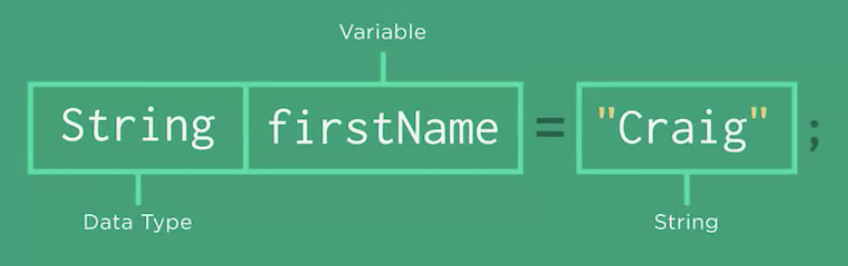
\includegraphics[width=0.7\linewidth]{images/part_1_1.png}
        \end{center}

        \item Are printed using \textit{console.printf()}
        \begin{itemize}
            \item i.e.

        \begin{lstlisting}[language=java]
        public class Introductions {
            public static void main(String[] args) {
                Console console = System.console();
                String firstName = "Ben";
                console.printf("Hello, my name is %s\n", firstName);
                console.printf("Craig is learning how to write Java\n");
            }
        }
        \end{lstlisting}
    \end{itemize}
\end{itemize}

\end{itemize}

\bigskip

\section{Exercise 1}

\bigskip

\begin{itemize}
    \item Solution included in \textit{exercise\_1.java}
\end{itemize}

\bigskip

\section{Receiving Input}

\bigskip

\begin{itemize}
    \item readline
    \begin{itemize}
        \item Receives input from user's end
        \item is in \textit{Console} object
        \item Is like \textit{stdin} in C or \textit{input} in Python

    \begin{lstlisting}[language=java]
    import java.io.Console;

    public class Introductions {
        public static void main(String[] args) {
            Console console = System.console();
            String firstName = console.readLine("What is your name?   "); // <- Here :)
            console.printf("Hello, my name is %s\n", firstName);
            console.printf("Craig is learning how to write Java\n");
        }
    }
    \end{lstlisting}
    \end{itemize}
\end{itemize}

\bigskip

\section{Exercise 2}

\bigskip

\begin{itemize}
    \item Solution included in \textit{exercise\_2.java}
\end{itemize}


\end{document}